\documentclass{beamer}
\usetheme{Berlin}
\usecolortheme{beaver}
\usepackage[utf8]{inputenc}
\usepackage[czech]{babel}
\usepackage{hyperref}

\setbeamerfont{page number in head/foot}{size=\small}
\setbeamertemplate{footline}[frame number]


\title
{Diplomová práce}
\subtitle{Inteligentní zabezpečovací systém garáže: nadřazený systém }
\author
{Ondřej Červenka \\ Vedoucí: Ing. Martin Daňhel}
\institute
{
  České vysoké učení technické v Praze\\
  Fakulta informačních technologií
}
\date{2018}

\begin{document}
  \frame{\titlepage}
  \begin{frame}
    \frametitle{Cíl práce}

    Cílem práce bylo navrhnout a implementovat nadřazený systém určený k zabezpečení garáže. Systém zbírá data od podřízených systémů umístěných v jednotlivých garážích.

    \hspace{1cm}

    Požadavky na systém:

    \begin{itemize}
      \item Komunikace s podřízenými systémy pomocí WiFi nebo Ethernetu.
      \item Webové uživatelské rozhraní pro správu.
      \item Reakce na události zaslané podřízenými systémy.
      \item Možnost provozu na jednodeskovém počítači (omezený HW).
    \end{itemize}
  \end{frame}

  \begin{frame}
    \frametitle{Návrh systému}

    \begin{figure}
        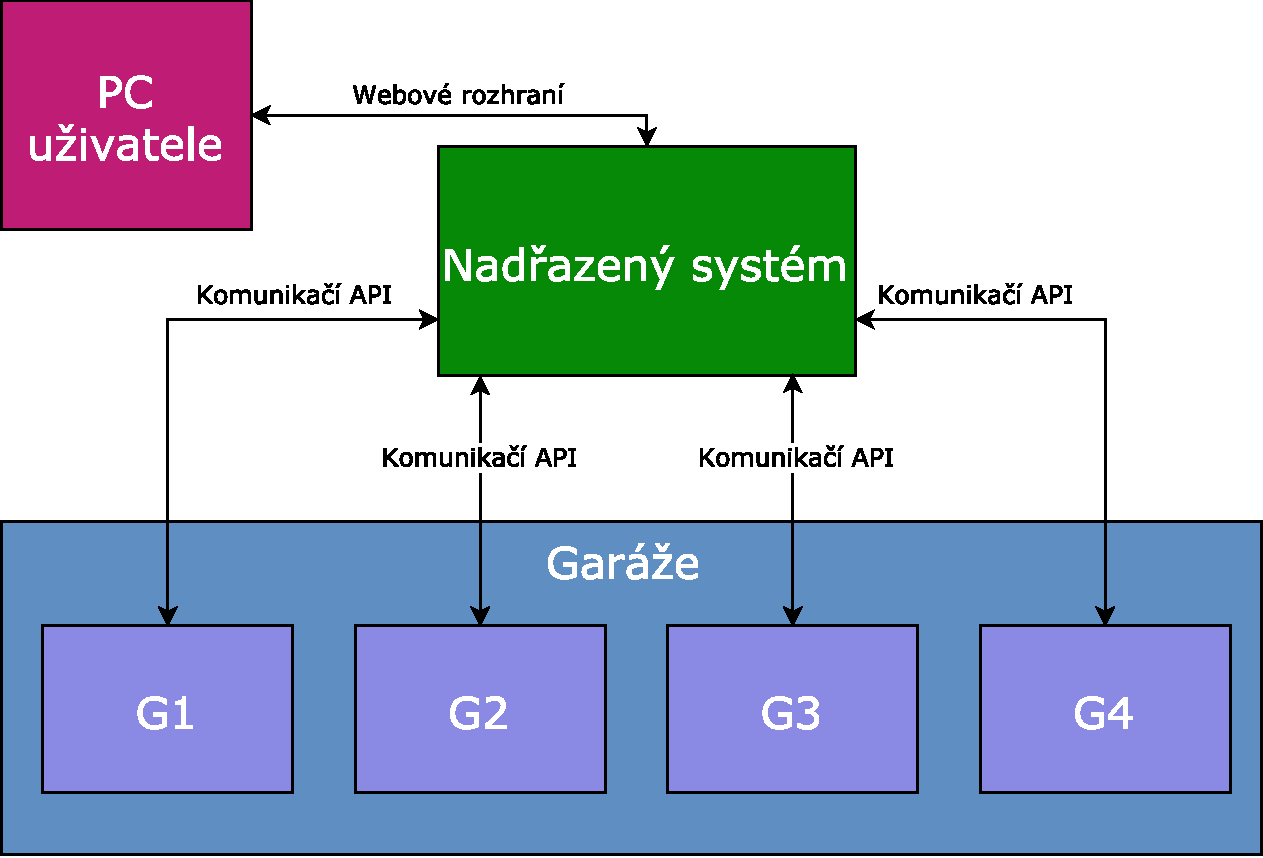
\includegraphics[scale=0.3]{../images/basic_struct.pdf}
        \caption{Základní struktura systému.}
      \end{figure}

      % popsat udalost a jak funguje to logovani dat
      % popsat ty ruzny udalosti vcetne tech kontrolnich hlaseni
  \end{frame}

  \begin{frame}
    \frametitle{Návrh systému}
    \framesubtitle{Komunikační protokol}

    Zkoumány byly protokoly HTTPS a MQTT z hlediska: 

    \begin{itemize}
      \item podpory na zvolené platformě (Raspberry Pi),
      \item zabezpečení. % u vobou ssl
    \end{itemize}

    Na základě této analýzi byl zvolen protokol HTTPS, na kterém bylo postaveno jednoduché API pro komunikaci s podřízenými systémy.

    % rict ze api primarne slouzi k zasilani udalosti vod podrizenejch systemu
    % tady říct, že to api slouží i k registraci/autorizaci systémů pomocí api klíčů.
    % taky rict ze duvody pro tuhle volbu bylo: jeden web server pro api i rozhrani, jednoduchost implementace

  \end{frame}

  \begin{frame}
    \frametitle{Návrh systému}
    \framesubtitle{Webové rozhraní}

    Webové rozhraní je určeno ke správě podřízených systémů a umožňuje:

    \begin{itemize}
      \item Registraci nových systému.
      \item Zobrazení zaznamenaných událostí.
      \item Editaci záznamu garáže (telefonní číslo, popis atp.).
      \item Změnu uživatelského nastavení.
    \end{itemize}

    Přístup do rozhraní je zabezpečen heslem. % tady zmínit ukládání hesla (hash)
    
  \end{frame}

  \begin{frame}
    \frametitle{Návrh systému}
    \framesubtitle{Reakce na události}

    Zasílání upozornění majiteli či nájemci při poplachu v garáži.
    % popsat to s tim zaslanim udalosti ktera zmeni stav, ze se posila upozorneni

    Zkoumané metody:

    \begin{itemize}
      \item E-mail -- pomocí Google GMail.
      \item SMS:
      \begin{itemize}
        \item GSM modul,
        \item služba Twilio. 
      \end{itemize}
    \end{itemize}

    % rict ze sem zkusil vsechno, zkoumal sem i to jak to bude slozity pro toho provozovatele zprovoznit (ruzny registrace atd.).
    % nakonec sem vybral gsm modul protoze jednoduchej, bez registrace a offline.
    % este rict ze ten gsm modul v zaklade potrebuje jen seriovou linku (zminit AT prikazy), tj ze se da pouzit na spouste jinejch platforem

  \end{frame}

  \begin{frame}
    \frametitle{Implementace}

    \begin{itemize}
      \item Programovací jazyk Python 3,
      \begin{itemize}
        \item webový framework Flask,
      \end{itemize}
      \item databázový systém SQLite 3,
      \item program Gammu pro ovládání GSM modulu.
    \end{itemize}

    % rict ze implementace byla primarne delana pro rpi, ale ze to de pouzit na v podstate libovolny platforme s temahle vecma

  \end{frame}

  \begin{frame}
    \frametitle{Testováni systému}

    \begin{itemize}
      \item Automatizované testy. % unit testy, dulezity pro dalsi rozsirovani
      \item Manuálni testy. % u tech smsek/gsm modulu
      \item Testovací nasazení.
      \item Simulátor podřízeného systému.
    \end{itemize}

  \end{frame}

  \begin{frame}
    \frametitle{Nasazení}

    \begin{figure}
        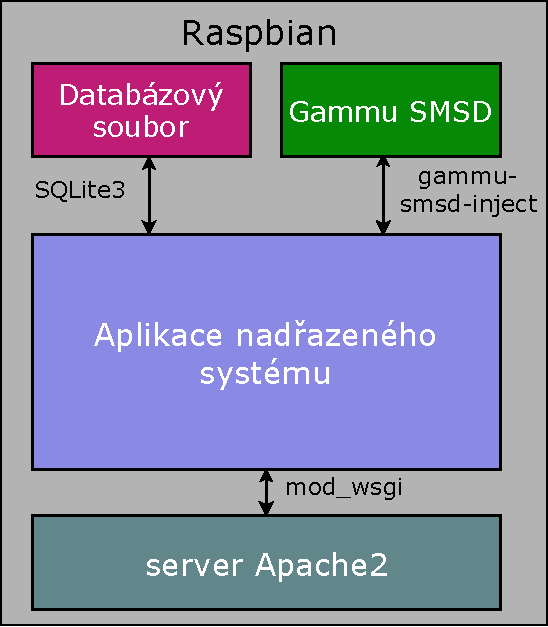
\includegraphics[scale=0.55]{../images/sw_block.pdf}
        \caption{Blokové schéma nasazeného systému.}
      \end{figure}
  \end{frame}

  \begin{frame}
    \frametitle{Závěr}

    Výsledky práce:

     \begin{itemize}
      \item Návrh a implementace nadřazeného systému,
      \item jeho otestování,
      \item nasazení na Raspberry Pi a virtuálním serveru.
     \end{itemize}
  \end{frame}

  \begin{frame}
    \frametitle{Otázky oponenta}

    Bylo by možné upravit webové rozhraní tak, aby podporovalo více uživatelů s různými právy? 

    Např. nájemce jedné z garáží by mít možnost sledovat události ve své garáži, případně upravovat telefonní číslo apod.

  \end{frame}

\end{document}
